\chapter{Cahier des charges}
\label{ch-cdc}

Ce chapitre fixe le cadre de l'étude : zone, norme et bande, équipements, objectifs et modèle de trafic. Chaque valeur est sourcée ; celles qui relèvent de notre jugement sont signalées comme hypothèses.

\section{La zone d'étude}
\label{sec-zone}

La zone couvre \num{10} × \SI{10}{\kilo\metre} en projection UTM 32N (EPSG:32632), de X = \SIrange{596}{606}{\kilo\metre} et Y = \SIrange{4022}{4032}{\kilo\metre}. Elle compte \num{25359} habitants d'après WorldPop 2020~\cite{worldpop2018}. L'occupation du sol, mesurée sur ESA WorldCover~\cite{worldcover2022}, se répartit en prairies (\SI{38,0}{\percent}), forêt (\SI{27,5}{\percent}), arbustes (\SI{13,3}{\percent}), cultures (\SI{13,0}{\percent}), bâti (\SI{6,6}{\percent}), sol nu (\SI{1,3}{\percent}) et eau (\SI{0,1}{\percent}).

Nous l'avons découpée en trois zones à partir des cartes (\cref{fig-zone,tab-zones}) :
\begin{itemize}
  \item le \textbf{centre urbain}, défini comme l'ensemble des pixels de \SI{100}{\metre} dont la densité atteint \SI{1000}{hab\per\kilo\metre\squared} ;
  \item le \textbf{massif}, au-dessus de \SI{600}{\metre} d'altitude : il correspond au parc national du Djebel Zaghouan, presque inhabité, où aucun site n'est autorisé et où nous ne fixons pas d'objectif ;
  \item la \textbf{zone rurale}, qui forme le reste.
\end{itemize}

\begin{figure}[H]
\centering
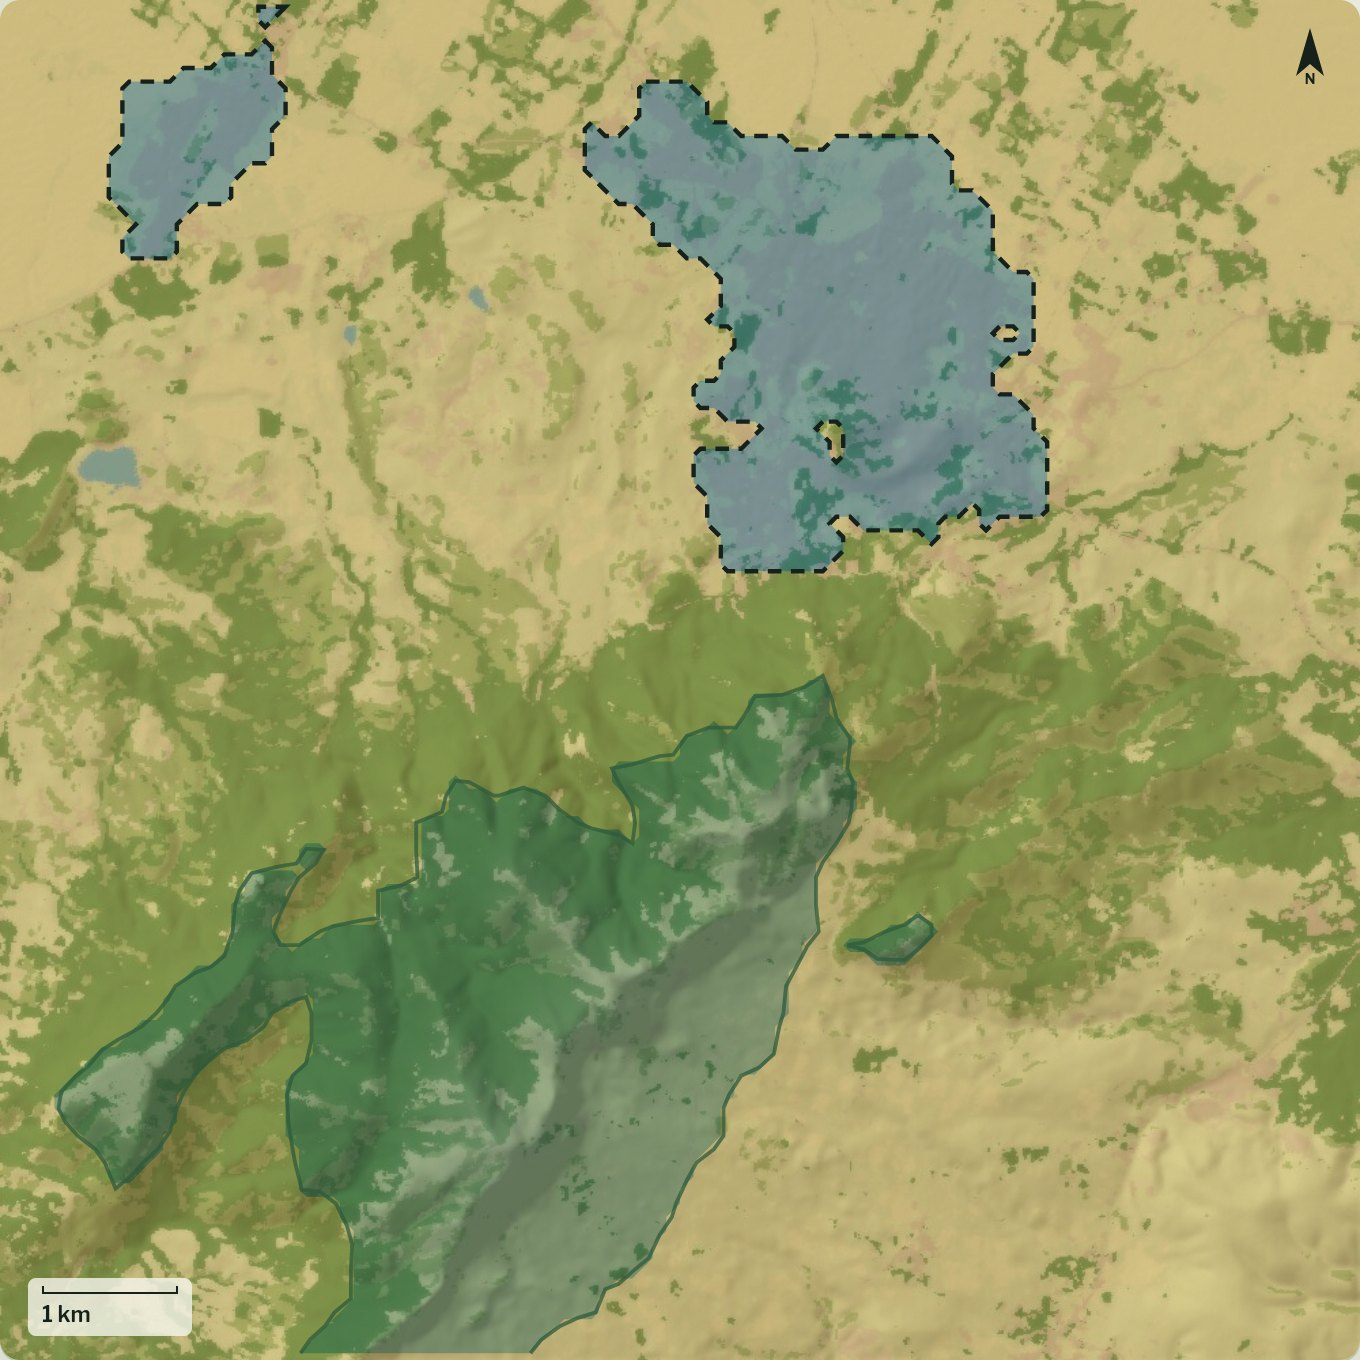
\includegraphics[width=0.62\textwidth]{zone.jpg}
\caption{Zone d'étude et découpage en trois zones.}
\label{fig-zone}
\end{figure}

La \cref{fig-zone} superpose l'occupation du sol (ESA WorldCover) au relief ombré (Copernicus). Le centre urbain est tracé en bleu, le massif au-dessus de \SI{600}{\metre} en vert foncé.

\begin{table}[H]
\centering
\caption{Les trois zones de l'étude.}
\label{tab-zones}
\begin{tabularx}{\textwidth}{@{}lLrrL@{}}
\toprule
\thead{Zone} & \thead{Définition} & \thead{Surface} & \thead{Habitants} & \thead{Stratégie} \\
\midrule
Centre urbain & densité $\geq$ \SI{1000}{hab\per\kilo\metre\squared} & \SI{8,57}{\kilo\metre\squared} & \num{13590} & capacité, objectif indoor \\
Rural & reste de la zone & \SI{76,95}{\kilo\metre\squared} & \num{11476} & couverture, objectif outdoor \\
Massif & altitude $\geq$ \SI{600}{\metre} & \SI{14,48}{\kilo\metre\squared} & \num{292} & aucun site, aucun objectif \\
\midrule
\textbf{Total} & & \SI{100}{\kilo\metre\squared} & \num{25359} & \\
\bottomrule
\end{tabularx}
\end{table}

\begin{cours}{objectif selon le contexte}
En zone urbaine ou suburbaine, l'objectif est d'assurer une capacité en trafic suffisante pour un grand nombre d'abonnés. En zone rurale, l'objectif est la couverture la plus complète possible, sans besoin de capacité élevée~\cite{afif2026cours}.
\application Le centre urbain est dimensionné par la capacité (§\,3.3 du sujet) et la campagne par la couverture (§\,3.2). Dans chaque zone, nous calculons quand même les deux besoins et gardons le plus grand (\cref{tab-sites-final}).
\end{cours}

\section{Choix de la norme}

\paragraph{LTE plutôt que GSM.} Le sujet demande des cartes de débit en liaison descendante (DL) et montante (UL) ainsi que des simulations Monte-Carlo. Dans Atoll 3.3, ces deux outils existent pour l'UMTS, le WiMAX et le LTE, mais pas pour le GSM. Nous avons retenu le LTE, la mieux documentée des trois~\cite{holma2011,sesia2011}. Le cours et le sujet sont rédigés dans la logique GSM (canaux, Erlang, motif de réutilisation) ; nous traduisons chaque étape en LTE au \cref{ch-dim}. En Tunisie, le LTE porte aussi l'essentiel du trafic : fin 2025, \SI{84}{\percent} des smartphones sont compatibles 4G et \SI{9}{\percent} compatibles 5G~\cite{intt2025tr4}.

\paragraph{Bande 3 (\SI{1800}{\mega\hertz}) plutôt que bande 20 (\SI{800}{\mega\hertz}).} Les deux bandes sont utilisées en Tunisie. La bande~20 ne fait que $2 × \SI{30}{\mega\hertz}$ pour trois opérateurs, soit au plus \SI{10}{\mega\hertz} chacun, alors que la bande~3 ($2 × \SI{75}{\mega\hertz}$) permet une porteuse de \SI{20}{\mega\hertz}~\cite{ts36101}. Le calcul du \cref{sec-800-1800} compare les deux bandes : le \SI{800}{\mega\hertz} porte plus loin et demande moins de sites aujourd'hui, mais sature en capacité quand le trafic augmente.

\begin{table}[H]
\centering
\caption{Norme et spectre retenus.}
\label{tab-norme}
\begin{tabularx}{\textwidth}{@{}lLl@{}}
\toprule
\thead{Paramètre} & \thead{Valeur} & \thead{Source} \\
\midrule
Norme & LTE (E-UTRA) FDD ; OFDMA en DL, SC-FDMA en UL & \cite{ts36211} \\
Bande & bande 3 : UL \SIrange{1710}{1785}{\mega\hertz}, DL \SIrange{1805}{1880}{\mega\hertz} & \cite{ts36101} \\
Porteuse & \SI{20}{\mega\hertz}, 100 blocs de ressources (RB) ; EARFCN 1300 : centre DL \SI{1815}{\mega\hertz}, UL \SI{1720}{\mega\hertz} & Atoll \\
Réutilisation & $K = 1$ : la même porteuse dans toutes les cellules (\cref{sec-reuse}) & calcul \\
\bottomrule
\end{tabularx}
\end{table}

\section{Équipements}

Les paramètres des équipements (\cref{tab-equip}) reprennent les modèles LTE fournis par Atoll, adaptés à notre porteuse de \SI{20}{\mega\hertz}. Les modèles de station d'Atoll sont prévus pour \SI{10}{\mega\hertz} et \SI{43}{\dBm}, ce qui donne une puissance par sous-porteuse du signal de référence (RS EPRE) de $43 - 10\log_{10} 600 = \SI{15,2}{\dBm}$. Pour garder cette puissance par sous-porteuse sur \num{1200} sous-porteuses, il faut $15{,}2 + 10\log_{10} 1200 = \SI{46}{\dBm}$. À puissance constante, doubler la bande ferait perdre \SI{3}{\deci\bel} par sous-porteuse.

\begin{table}[H]
\centering
\caption{Paramètres des équipements.}
\label{tab-equip}
\begin{tabularx}{\textwidth}{@{}lLl@{}}
\toprule
\thead{Paramètre} & \thead{Valeur} & \thead{Source} \\
\midrule
Puissance de l'eNodeB & \SI{46}{\dBm} (\SI{40}{\watt}) sur \SI{20}{\mega\hertz} & Atoll, calcul \\
Facteur de bruit de l'eNodeB & \SI{5}{\deci\bel} & Atoll \\
Antenne & tri-secteur \ang{65}, \SI{18}{\dBi} ; à \SI{30}{\metre} ; tilt électrique \ang{4} (urbain), \ang{2} (rural) ; MIMO 2 × 2 & Atoll \\
Pertes d'émission et de réception & \SI{1}{\deci\bel} (tête radio déportée en haut du mât) & hypothèse \\
Puissance du terminal & \SI{23}{\dBm} (classe de puissance 3) & \cite{ts36101} \\
Facteur de bruit du terminal & \SI{8}{\deci\bel} ; gain d'antenne \SI{0}{\dBi} & Atoll \\
Perte de corps & \SI{3}{\deci\bel} en VoIP, \SI{0}{\deci\bel} en données & Atoll \\
\bottomrule
\end{tabularx}
\end{table}

Le choix d'une tête radio déportée en haut du mât ramène les pertes de câble à environ \SI{1}{\deci\bel}, au lieu d'environ \SI{2,3}{\deci\bel} pour \SI{30}{\metre} de câble coaxial ; un amplificateur de mât devient alors inutile.

\section{Objectifs de couverture et de qualité}
\label{sec-objectifs}

\begin{table}[H]
\centering
\caption{Objectifs du cahier des charges.}
\label{tab-objectifs}
\begin{tabularx}{\textwidth}{@{}lL@{}}
\toprule
\thead{Objectif} & \thead{Valeur} \\
\midrule
Couverture du centre urbain & \SI{95}{\percent} de la surface, \textbf{en indoor} \\
Couverture de la campagne & \SI{95}{\percent} de la surface, \textbf{en outdoor} \\
Massif & aucun objectif \\
Débit en bord de cellule & \SI{1024}{\kbps} en DL, \SI{128}{\kbps} en UL \\
Charge maximale d'une cellule à l'heure chargée & \SI{80}{\percent} \\
\bottomrule
\end{tabularx}
\end{table}

Le débit visé en bord de cellule est celui du service \enquote{High Speed Internet} d'Atoll (\SI{1024}{\kbps} en DL, \SI{128}{\kbps} en UL), ce qui permet de le vérifier directement sur les cartes de débit et dans les simulations. Le bearer le plus robuste accepté par ce service est le bearer~4 (QPSK 1/3), avec un seuil de SINR de \SI{-1}{\deci\bel} dans Atoll : c'est la qualité minimale à garantir en bord de cellule. La charge maximale de \SI{80}{\percent} joue en LTE le rôle du taux de blocage de la loi d'Erlang~B, en gardant une réserve dans chaque cellule.

\section{Modèle de trafic}
\label{sec-trafic}

Les données de marché viennent du tableau de bord de l'INTT pour le quatrième trimestre 2025~\cite{intt2025tr4}.

\begin{table}[H]
\centering
\caption{Hypothèses de trafic.}
\label{tab-trafic}
\begin{tabularx}{\textwidth}{@{}lLl@{}}
\toprule
\thead{Paramètre} & \thead{Valeur} & \thead{Source} \\
\midrule
Pénétration de la data mobile & \SI{93,9}{\percent} par habitant & \cite{intt2025tr4} \\
Part de marché de l'opérateur & \SI{30}{\percent}, part médiane des trois opérateurs (\SI{43,5}{\percent}, \SI{30,4}{\percent}, \SI{25,8}{\percent}) & \cite{intt2025tr4} \\
Terminaux compatibles LTE & \SI{93}{\percent} (\SI{84}{\percent} 4G + \SI{9}{\percent} 5G) & \cite{intt2025tr4} \\
Volume de données & \SI{9,5}{Go} par abonné et par mois (\SI{6,8}{Go} fin 2023) & \cite{intt2025tr4} \\
Part de l'heure chargée & \SI{10}{\percent} du trafic journalier & hypothèse \\
Répartition DL / UL & \SI{90}{\percent} / \SI{10}{\percent} & hypothèse \\
\bottomrule
\end{tabularx}
\end{table}

Le débit moyen d'un abonné à l'heure chargée vaut donc
\begin{equation}
  \frac{\SI{9,5}{Go} × 8}{30~\text{jours}} × \SI{10}{\percent} × \frac{1}{\SI{3600}{\second}} \approx \SI{70,4}{\kbps},
\end{equation}
dont \SI{63,3}{\kbps} en DL et \SI{7,0}{\kbps} en UL. Le volume mensuel a augmenté d'environ \SI{40}{\percent} en deux ans (de 6,8 à \SI{9,5}{Go}) : nous utilisons ce rythme pour vérifier que le réseau tient dans cinq ans.
